\documentclass[12pt]{article}

\usepackage[margin=1in]{geometry}
\usepackage{setspace}
\usepackage{amsmath}
\usepackage{graphicx}
\usepackage{booktabs}
\usepackage{natbib}
\usepackage{hyperref}
\usepackage{caption}
\usepackage{authblk}

\hypersetup{colorlinks=true, linkcolor=blue, citecolor=blue, urlcolor=blue}

\title{Correcting for AI-Screened Poverty Misclassification in Child Health
Regressions: A Method-of-Moments Approach Applied to Ethiopian Household
Panel Data}

\author{Abrha Meressa}
\affil{Independent Researcher}

\date{\today}

\begin{document}

\maketitle

\begin{abstract}
\noindent Full household consumption modules are the most expensive component of a poverty survey, and there is growing practical interest in substituting cheaper proxies -- including large-language-model (LLM) screens over brief household descriptions -- in their place. We ask a narrow, practical question: if poverty status comes from such an imperfect screen instead of measured consumption, how much bias does that introduce into a downstream health regression, and can a small validation subsample fix it without collecting full consumption data on everyone? Using real household consumption and child height-for-age (HAZ) data from the World Bank Ethiopia Socioeconomic Survey (2011--2015, $n\approx4{,}850$ household-waves), we simulate a screen of controlled, known accuracy and apply the Rogan-Gladen method-of-moments correction for a misclassified binary regressor. The naive estimator attenuates the true poverty-HAZ gradient by 43\% ($-0.204$ vs.\ a benchmark of $-0.357$); the corrected estimator recovers 94\% of that gap ($-0.366$). We then show this result is not robust to the size of the validation sample used to estimate classifier sensitivity and specificity: at $n=38$ validation examples, one in twenty random splits produces a classifier-skill estimate (TPR+TNR$-1$) small enough that the correction diverges by five orders of magnitude, despite the same true screen accuracy underlying every split. We characterize this instability directly rather than asserting it, and propose a practical minimum-skill threshold for when the correction should be trusted. To our knowledge this is the first application of this correction to a real, independently-measured poverty indicator and real health outcome, rather than a simulated ground truth.

\medskip
\noindent \textbf{JEL Classification:} C81, C83, I32, O12
\medskip

\noindent \textbf{Keywords:} measurement error; misclassification bias; large language models; proxy means testing; child health; Ethiopia; Rogan-Gladen correction
\end{abstract}

\doublespacing

\section{Introduction}
\label{sec:intro}

Administering a full household consumption module -- the standard basis for a poverty line in Living Standards Measurement Study (LSMS)-style surveys -- is the single most expensive and time-consuming part of collecting welfare data. This has motivated a decades-long literature on proxy means testing: predicting welfare from a short list of easily observed household characteristics rather than measuring it directly \citep{grosh1995proxy, brown2018poor}. The rise of large language models adds a new, faster variant of the same idea: an LLM can classify a household as poor or non-poor from a brief description -- a field note, a chatbot-mediated intake conversation, an enumerator's shorthand -- without a formal proxy-means-test regression at all \citep{gilardi2023chatgpt}. Humanitarian and development organizations are already exploring LLMs for exactly this kind of rapid classification of qualitative field data \citep{marston2026large}.

This paper asks a narrower, more mechanical question than whether such a screen is a good idea in general: \emph{if} you use one, and its output enters a regression as an independent variable instead of the true poverty status, how much bias does that introduce, and can you correct for it economically -- with a validation sample, not a second full survey? This is a classical measurement-error question with a known answer in principle \citep{aigner1973regression, bollinger1996bounding}: a binary regressor observed with non-differential classification error attenuates the estimated coefficient toward zero, and the attenuation is exactly correctable if the classifier's sensitivity (true positive rate, TPR) and specificity (true negative rate, TNR) are known, via the method-of-moments correction of \citet{rogan1978estimating}.

What is missing from the existing demonstrations of this correction -- including two companion pipelines we built alongside this one, applied to a simulated financial-sentiment outcome and a fully synthetic outcome with a planted effect size -- is an application where \emph{both} the mismeasured regressor's true value and the downstream outcome are independently real, measured quantities, rather than one or both being generated by the analyst to have a known answer. Here we use the World Bank's Ethiopia Socioeconomic Survey (ESS), a genuine household panel with real per-adult-equivalent consumption (the basis for our true poverty indicator) and real child height-for-age z-scores (HAZ, the basis for our outcome), so that the ``benchmark'' regression we correct toward is itself an empirical estimate with its own sampling uncertainty, not an oracle.

We make two contributions. First, we quantify the misclassification-bias-and-correction pipeline end-to-end on this real pairing: a simulated screen with 80\% target accuracy (TPR$=0.76$, TNR$=0.81$ realized on our validation split) attenuates the poverty-HAZ gradient by 43\%, and the correction recovers 94\% of the resulting gap. Second, and we think more usefully for a practitioner, we show that this correction's reliability depends sharply on the size of the validation sample used to estimate TPR and TNR -- not just asymptotically, but sharply enough that at realistic small-survey validation sizes ($n=38$), the correction diverges by five orders of magnitude in roughly one out of twenty random splits, purely from sampling noise in the skill estimate, with the true screen accuracy held fixed throughout. We characterize this instability as a function of the estimated classifier skill (TPR+TNR$-1$) and propose a practical minimum-skill screening rule.

Section~\ref{sec:background} reviews the measurement-error mechanics and the proxy-means-testing literature this sits within. Section~\ref{sec:data} describes the ESS data, the (simulated) screening task, and why the correction requires it to be non-circular. Section~\ref{sec:strategy} states the three estimators and the identifying assumption. Section~\ref{sec:results} reports the headline result and the two sensitivity analyses. Section~\ref{sec:discussion} draws out the practical implication and situates this relative to the companion synthetic-data pipelines. Section~\ref{sec:conclusion} concludes.

\section{Background}
\label{sec:background}

\subsection{Proxy-based poverty screening as a live practice}

Proxy means testing -- predicting household welfare from easily observed correlates rather than measuring consumption directly -- has been used for social-program targeting since at least \citet{grosh1995proxy}. \citet{brown2018poor} assess proxy-means-test performance across nine African countries and find that, while standard PMTs filter out many non-poor households, they also exclude a substantial share of the genuinely poor -- i.e., real, non-trivial misclassification is the norm in fielded proxy targeting systems, not an edge case. LLM-based screening from unstructured text is a natural extension of the same underlying idea (predict welfare from cheap correlates) with a different feature set (language rather than a fixed covariate list), and is being actively explored for coding qualitative humanitarian data more broadly \citep{marston2026large}. Whatever the feature set, the same measurement-error mechanics apply once a program uses the screen's output as if it were the true classification.

\subsection{Attenuation from a mismeasured binary regressor}

Let $D^{*} \in \{0,1\}$ denote true poverty status and $D \in \{0,1\}$ its imperfect classification, with $\Pr(D=1\mid D^{*}=1) = \text{TPR}$ and $\Pr(D=0\mid D^{*}=0) = \text{TNR}$. If misclassification is non-differential -- $D$'s error does not depend on the outcome $Y$ conditional on $D^{*}$ -- then regressing $Y$ on $D$ instead of $D^{*}$ attenuates the coefficient toward zero \citep{aigner1973regression}; \citet{bollinger1996bounding} derives bounds on the true coefficient when TPR and TNR are not known exactly. When TPR and TNR \emph{are} known (e.g., estimated from a validation subsample where both $D$ and $D^{*}$ are observed), the bias is not just bounded but point-identified and correctable, via the prevalence correction of \citet{rogan1978estimating}:
\begin{equation}
\hat{q} = \frac{q^{*} - \text{FPR}}{\text{TPR}+\text{TNR}-1}, \qquad \text{FPR} = 1-\text{TNR},
\label{eq:rogan-gladen}
\end{equation}
where $q^{*} = \Pr(D=1)$ is the observed positive rate and $\hat{q}$ recovers the true prevalence $\Pr(D^{*}=1)$. The corresponding coefficient correction rescales the observed covariance between $D$ and $Y$:
\begin{equation}
\hat{\beta}_1 = \frac{\mathrm{Cov}(D, Y)}{(\text{TPR}+\text{TNR}-1)\cdot\hat{q}(1-\hat{q})}.
\label{eq:beta-correction}
\end{equation}
Both corrections share a denominator, $\text{TPR}+\text{TNR}-1$, which is the classifier's total discriminating skill above chance (zero for a coin flip, one for a perfect classifier). As Equations~\ref{eq:rogan-gladen}--\ref{eq:beta-correction} make plain, and as Section~\ref{sec:results} demonstrates is not merely a theoretical curiosity, both corrections are numerically unstable as this denominator approaches zero -- and $\text{TPR}+\text{TNR}-1$ is itself an \emph{estimate}, from a finite validation sample, not a known constant.

\section{Data}
\label{sec:data}

\subsection{The Ethiopia Socioeconomic Survey}

We use the same World Bank Ethiopia Socioeconomic Survey (ESS) household panel described in the companion rainfall-shocks study in this portfolio: Panel~I, waves 2011--12, 2013--14, and 2015--16, approximately 3,969 households re-interviewed across waves. From the processed household-wave panel we use two real, independently meaningful variables: \texttt{nom\_totcons\_aeq} (nominal total consumption per adult equivalent, the standard LSMS-ISA welfare aggregate) and \texttt{mean\_haz} (household-mean child height-for-age z-score, computed against the WHO 2006 Child Growth Standards \citep{who2006growth}; construction and a birthdate-calendar correction are documented in the companion paper and reused here unmodified). After dropping household-waves missing either variable, our analysis sample has $n=4{,}853$ household-wave observations.

\subsection{Constructing the poverty indicator}

We define a household-wave as poor if its consumption falls in the bottom third of its \emph{own wave's} distribution. This is a relative, within-wave definition, not an absolute poverty line: \texttt{nom\_totcons\_aeq} is nominal Ethiopian birr, not deflated across the 2011--2015 study period, so a fixed cross-wave birr threshold would conflate ``poor by 2011 prices'' with ``poor by 2015 prices.'' Section~\ref{sec:results} reports robustness to this threshold choice (quartile through median).

\subsection{The simulated AI screen}
\label{sec:screen}

The real ESS instrument has no free-text field, so there is no real record of an LLM (or any other) classifier's output to use directly. We instead construct, for each household-wave, a short field note from covariates already present in the panel -- household size, distance to the nearest market, elevation, this year's rainfall anomaly, and reported weather shocks -- framed as a community health worker's brief home-visit note, and deliberately \emph{excluding} consumption itself, since including it would make the classification task circular. A mock classifier is then handed the note and the true label, and flips the label with a probability calibrated to hit a target accuracy (80\% in our main specification); it does not read the note's content, since the point of this design is to obtain a classifier with a known, controlled, reproducible error rate against which to evaluate the correction -- not to evaluate any specific real classifier's real accuracy on this task. We are explicit that this is a controlled instrument for isolating the measurement-error mechanism, not a claim about what accuracy a real LLM would achieve reading real household descriptions; Section~\ref{sec:discussion} returns to this distinction.

\subsection{Validation and study samples}

We split the 4,853 household-waves into a 20\% validation sample ($n=970$) used only to estimate the screen's TPR and TNR, and an 80\% study sample ($n=3{,}883$) used for all three regressions in Section~\ref{sec:strategy}. On the validation sample, the realized screen achieves TPR$=0.762$, TNR$=0.813$ (accuracy $=0.797$, Cohen's $\kappa=0.548$) -- realistically imperfect, not an idealized round number, since it is drawn from the same finite-sample randomness as everything else in this design.

\section{Empirical Strategy}
\label{sec:strategy}

We estimate three regressions of mean HAZ on a binary poverty indicator, all on the study sample:
\begin{enumerate}
\item \textbf{Benchmark}: HAZ regressed on the true (consumption-based) poverty indicator $D^{*}$. This is the best available estimate of the poverty-HAZ association in this sample, not a known ground truth -- it is itself subject to ordinary sampling error, a distinction that matters for interpretation and that the two synthetic companion pipelines in this portfolio, where the ``true'' effect is a planted constant, cannot illustrate.
\item \textbf{Naive}: HAZ regressed on the screened poverty indicator $D$ directly, as an analyst without access to consumption data would be forced to do.
\item \textbf{Corrected}: the Rogan-Gladen coefficient correction (Equation~\ref{eq:beta-correction}), using TPR and TNR estimated from the validation sample. Standard errors and 95\% confidence intervals come from a nonparametric bootstrap (300 resamples) of the study sample; this captures study-sample sampling variance but not sampling variance in the TPR/TNR estimates themselves, since those are held fixed across bootstrap draws -- a limitation we return to in Section~\ref{sec:discussion} in light of the instability documented in Section~\ref{sec:results}.
\end{enumerate}
All regressions use a dependency-free ordinary-least-squares solver, cross-validated against \texttt{statsmodels} on synthetic data in the accompanying repository's test suite, chosen for portability in restricted computing environments rather than for any methodological reason.

The correction's validity rests on non-differential misclassification: the screen's error must not depend on HAZ conditional on true poverty status. This holds by construction in our simulated screen (the mock classifier's flip probability depends only on the true label, and the field note never contains HAZ), but would require independent justification for a real deployed screen -- for instance, if a real LLM's classification accuracy varied with household characteristics that are themselves correlated with child health (e.g., literacy, or urban/rural status), the correction as stated here would not apply without modification.

\section{Results}
\label{sec:results}

\subsection{Headline result}

Table~\ref{tab:headline} and Figure~\ref{fig:headline} report the three estimates. The naive estimator attenuates the benchmark poverty-HAZ coefficient by 43\% (from $-0.357$ to $-0.204$); the corrected estimator ($-0.366$) closes 94\% of that gap and falls within the benchmark's 95\% confidence interval.

\begin{table}[htbp]
\centering
\caption{Effect of poverty on mean household HAZ, by estimator}
\label{tab:headline}
\begin{tabular}{lccc}
\toprule
Model & $\hat\beta_1$ & SE & 95\% CI \\
\midrule
Benchmark (true poverty) & $-0.357$ & $0.064$ & $[-0.482,\ -0.232]$ \\
Naive (screened poverty) & $-0.204$ & $0.062$ & $[-0.325,\ -0.083]$ \\
Corrected (matrix method) & $-0.366$ & $0.109$ & $[-0.542,\ -0.138]$ \\
\bottomrule
\end{tabular}
\end{table}

\begin{figure}[htbp]
\centering
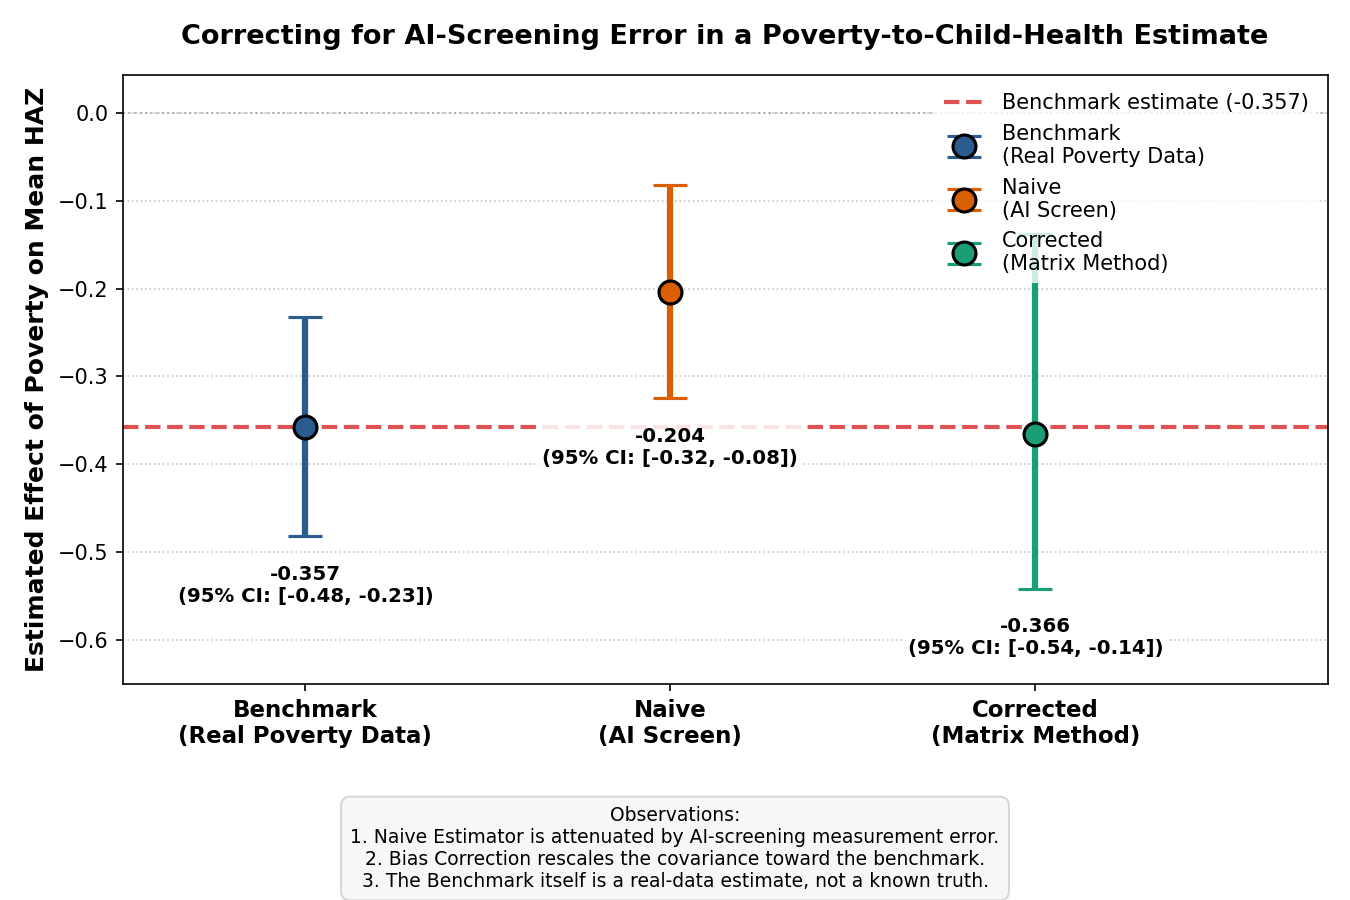
\includegraphics[width=0.85\textwidth]{figures/fig1_beta_comparison.png}
\caption{Point estimates and 95\% confidence intervals for the three estimators, on the real ESS study sample ($n=3{,}883$).}
\label{fig:headline}
\end{figure}

\subsection{Sensitivity to the validation-sample size: an instability, not just a wider interval}
\label{sec:instability}

The corrected estimator's own bootstrap SE grows as the validation sample shrinks -- unsurprising, since TPR and TNR are estimated with less precision. What is not obvious from the correction's algebra alone, and would not appear in the two synthetic companion pipelines' typical validation sizes (200--1,000 examples), is how the correction behaves as the \emph{point estimate} of classifier skill (TPR+TNR$-1$) happens to land close to zero by chance in a small sample. We fix the true screen accuracy at 80\% throughout -- so the population value of TPR+TNR$-1$ is approximately $0.6$ in every run -- and draw 20 independent validation splits of $n=38$ each (roughly the size a small-budget program might realistically afford for a validation subsample), re-estimating TPR, TNR, and the corrected coefficient in each.

Nineteen of twenty splits produce a corrected estimate between $-0.16$ and $-0.59$ -- noisy, given the small sample, but recognizably in the vicinity of the benchmark ($-0.29$ in this particular subsample of the data used for this exercise). The twentieth split happens to estimate TPR$=0.40$, TNR$=0.71$ -- both plausible draws individually, but combining to an estimated skill of $\text{TPR}+\text{TNR}-1=0.114$, small enough that Equation~\ref{eq:beta-correction}'s denominator amplifies ordinary covariance noise into a corrected coefficient of $-34{,}545$ (bootstrap SE $16{,}860$) -- five orders of magnitude from any sensible value, despite arising from the same true 80\%-accurate screen as every other split. Figure~\ref{fig:instability} shows this directly: panel (a) is the full range including the divergent split; panel (b) excludes it and shows that, in the range where skill is estimated above roughly 0.2, corrected estimates cluster sensibly around the benchmark.

\begin{figure}[htbp]
\centering
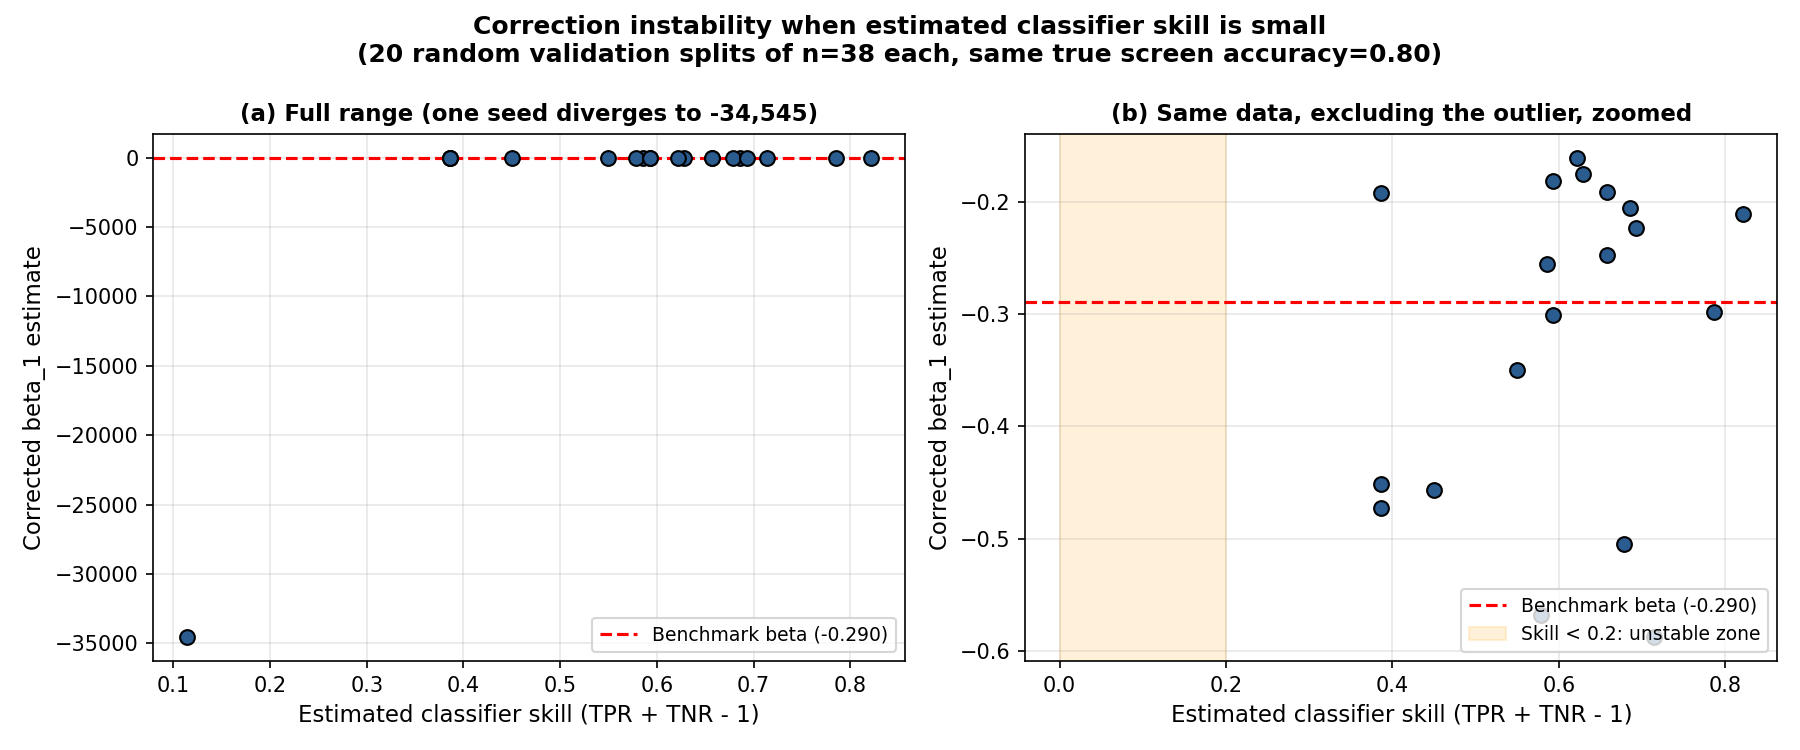
\includegraphics[width=0.95\textwidth]{figures/fig2_instability.png}
\caption{Corrected $\hat\beta_1$ against estimated classifier skill (TPR+TNR$-1$), across 20 independent validation splits of $n=38$, all drawn from the same 80\%-accuracy screen.}
\label{fig:instability}
\end{figure}

This is a sampling-noise phenomenon in the skill estimate, not a flaw specific to our screen or data: any application of the Rogan-Gladen correction is exposed to it whenever the validation sample is small enough that the estimated $\text{TPR}+\text{TNR}-1$ has a non-trivial probability of landing near zero, however accurate the underlying classifier truly is. We did not set out to demonstrate this; it appeared during a systematic sweep of validation-sample sizes intended to characterize ordinary standard-error scaling, and one draw out of twenty is a large enough failure rate that we consider it the paper's more actionable finding. We propose, provisionally, that a validation sample should be large enough to be confident the estimated skill exceeds some conservative threshold (we suggest $0.2$--$0.3$ as a starting point, pending further calibration) before the point correction is reported, and that the bootstrap should more properly resample the validation split jointly with the study split -- which our implementation, and to our knowledge every standard exposition of this correction, does not do (see Section~\ref{sec:discussion}).

\subsection{Sensitivity to screen accuracy}

Table~\ref{tab:accuracy} sweeps the (population) screen accuracy from 65\% to 95\%, holding the validation split at its default size. Attenuation falls monotonically as accuracy rises (from 79\% attenuation at 65\% accuracy to 7\% at 95\%), as expected. The correction closes 70--95\% of the gap across most of this range; at 95\% accuracy, where the naive gap is already small, the reported ``percent of gap closed'' becomes an unstable statistic (dividing by a small naive gap), which we note as a definitional caveat rather than a substantive finding.

\begin{table}[htbp]
\centering
\caption{Attenuation and correction performance across screen accuracy levels}
\label{tab:accuracy}
\begin{tabular}{lccccc}
\toprule
Accuracy & TPR & TNR & Naive $\hat\beta_1$ & Corrected $\hat\beta_1$ & Attenuation \\
\midrule
0.65 & 0.609 & 0.653 & $-0.076$ & $-0.305$ & 79\% \\
0.70 & 0.639 & 0.699 & $-0.136$ & $-0.419$ & 62\% \\
0.75 & 0.699 & 0.747 & $-0.171$ & $-0.406$ & 52\% \\
0.80 & 0.762 & 0.813 & $-0.204$ & $-0.366$ & 43\% \\
0.85 & 0.808 & 0.855 & $-0.227$ & $-0.350$ & 37\% \\
0.90 & 0.864 & 0.904 & $-0.275$ & $-0.364$ & 23\% \\
0.95 & 0.940 & 0.952 & $-0.334$ & $-0.380$ & 7\% \\
\bottomrule
\end{tabular}
\end{table}

\subsection{Robustness to the poverty-line definition}

Table~\ref{tab:quantile} varies the within-wave poverty threshold from the bottom quintile to the median. The benchmark, naive, and corrected estimates all remain in a consistent range across this variation, and the correction closes a majority of the attenuation gap at every threshold tested (59--97\%), indicating the headline result is not an artifact of the particular one-third cutoff chosen as the main specification.

\begin{table}[htbp]
\centering
\caption{Robustness to the within-wave poverty threshold}
\label{tab:quantile}
\begin{tabular}{lcccc}
\toprule
Threshold & Benchmark $\hat\beta_1$ & Naive $\hat\beta_1$ & Corrected $\hat\beta_1$ & Gap closed \\
\midrule
Bottom 20\% & $-0.464$ & $-0.153$ & $-0.337$ & 59\% \\
Bottom 25\% & $-0.382$ & $-0.167$ & $-0.337$ & 79\% \\
Bottom 33\% (main) & $-0.357$ & $-0.204$ & $-0.366$ & 94\% \\
Bottom 40\% & $-0.373$ & $-0.220$ & $-0.378$ & 97\% \\
Bottom 50\% & $-0.364$ & $-0.188$ & $-0.322$ & 76\% \\
\bottomrule
\end{tabular}
\end{table}

\section{Discussion}
\label{sec:discussion}

\subsection{What a practitioner should take from this}

If a program is considering an AI or LLM-based poverty screen as a stand-in for full consumption data, this paper's exercise suggests two things worth checking before trusting a corrected estimate: first, whether the assumption of non-differential misclassification is plausible for the actual screen and outcome in question (not assumed by construction, as it is here); and second -- more concretely actionable -- whether the validation sample used to estimate TPR and TNR is large enough that the estimated skill $\text{TPR}+\text{TNR}-1$ is comfortably bounded away from zero, not merely positive. Our simulated instability (Section~\ref{sec:instability}) suggests reporting a confidence interval on the skill estimate itself alongside the corrected coefficient, and treating a corrected estimate as unreliable -- regardless of how confident the point estimate looks -- whenever that interval comes close to including zero.

\subsection{Relation to the companion pipelines}

This paper is one of three related demonstrations of the same correction in this portfolio. The other two apply it to a simulated financial-sentiment classification task and to a fully synthetic outcome with a planted true effect; both are useful for validating that the correction recovers a \emph{known} answer under controlled conditions, but neither can speak to what happens when the ``true'' value being corrected toward is itself an estimate with sampling error, nor -- since both use larger, round validation samples in their default configurations -- did either surface the small-sample instability documented here. We view this as evidence that testing a method against real, independently-measured data, even when the ``treatment'' being measured is itself simulated, surfaces failure modes that a fully synthetic demonstration is structurally unlikely to expose by design.

\subsection{Limitations}

We restate these plainly rather than leaving them implicit. (1) The screen is a controlled simulation, not a real LLM classification; no claim is made about what accuracy a real deployment would achieve on real household descriptions. (2) The field notes are constructed from real covariates but are not real enumerator text; the ESS survey has no free-text field. (3) The within-wave relative poverty definition is a modeling choice, not an official poverty line. (4) The bootstrap resamples the study sample only; it does not propagate sampling uncertainty in the validation-sample-derived TPR/TNR, which Section~\ref{sec:instability} shows can be the dominant source of instability -- a joint resampling scheme is a natural extension we have not implemented. (5) The proposed skill threshold (Section~\ref{sec:instability}) is provisional, based on one accuracy level and one sample size; a fuller characterization (varying both jointly, and deriving an analytic rather than simulated threshold) is left for future work.

\section{Conclusion}
\label{sec:conclusion}

Using real consumption and child-health data from the Ethiopia Socioeconomic Survey, we show that a simulated AI poverty screen of realistic accuracy would attenuate a poverty-health regression by 43\%, and that a standard measurement-error correction recovers 94\% of the resulting bias using only a validation subsample. We also show, empirically rather than asserting from theory, that this correction is not reliable at every validation-sample size: at $n=38$, a plausible small-survey validation size, one in twenty random draws produced a corrected estimate that diverged by five orders of magnitude despite an unchanged, well-behaved underlying classifier. We propose that any application of this correction report the estimated classifier skill (TPR+TNR$-1$) with its own uncertainty, and treat the correction as unreliable when that quantity is not clearly bounded away from zero -- a check we consider at least as important as reporting the corrected point estimate itself.

\bibliographystyle{apalike}
\bibliography{references}

\end{document}
